\documentclass[11pt,a4paper,UKenglish]{memoir}
% Template by DTU LaTeX support group, v20090423

\usepackage[utf8]{inputenc} % Must correspond to the input encoding used by the editor
\usepackage{babel} % Other languages, in this case UKenglish
\usepackage[T1]{fontenc} % font encoding (output), use T1 for most latin languages
\usepackage{lmodern} % vector based Computer Modern font
\usepackage{graphicx} % for graphics
\graphicspath{{./figures/}} % path to figures and images

\usepackage{mathtools} % mathmatics

\usepackage{xcolor}
\usepackage[plainpages=false,pdfpagelabels,pageanchor=false]{hyperref} % active links
\hypersetup{%
  pdfauthor={
  	Dzitkowski Karol \\
	Marco Becattini},
  pdftitle={02450 Project 1},
  pdfsubject={Introduction to Machine Learning and Data Mining},
  citebordercolor={0 1 0}, % The color of the box around citations (change to 1 1 1 to remove)
  linkbordercolor={1 0 0}, % The color of the box around normal links
  pagebordercolor={1 1 0}, % The color of the box around links to pages
  urlbordercolor= {1 1 1}  % The color of the box around links to URLs
}
\usepackage{memhfixc}% fixes for hyperref

% The following can be used if not using custom frontpage
\title{02450 Project 1}
\author{
	Dzitkowski Karol \\
	Marco Becattini
}
\date{\today}%

% \includeonly{preface,testing} % Only compile those files you are working in (to save compile time, and power)

\begin{document}
\frontmatter % roman page numbering
%\maketitle  % use this if not using custom frontpage


\begin{titlingpage}
\centering \parindent=0pt
\newcommand{\HRule}{\rule{\textwidth}{1mm}}
\vspace*{\stretch{1}} \HRule\\[1cm]\Huge\bfseries
02450 Project 3\\[0.7cm]
\large Report\\[1cm]
\HRule\\[4cm]  
\large by Karol Dzitkowski\\
Marco Becattini\\
\vspace*{\stretch{2}} \normalsize %
\begin{flushleft}
Technical University of Denmark\\
Department of Applied Mathematics and Computer Science\\
Introduction to Machine Learning and Data Mining\\
Tue Herlau\\
\today \end{flushleft}
\end{titlingpage}


\begin{abstract}
The objective of this second report is to apply the methods you have learned in the second section of the course on ,,Supervised learning: Classification and regression'' in order to solve both a relevant classification and regression problem for your data.
\end{abstract}


%\tableofcontents
%\listoffigures
%\listoftables

\mainmatter % arabic page numbering

%In this report we apply regression and classification to the "Letter Image Recognition" dataset
\chapter*{Regression}
\setcounter{chapter}{1}
\section*{1.1 Problem}
\setcounter{section}{1}
Let D denote our data set that contains N observations:
\begin{center}
$D = \{( \textbf{x}_i ,y_i ) | i = 1, 2, \dots, N\}$
\end{center}
Each $\textbf{x}_i $ corresponds to the set of attributes of the $i$-th observation and $y_i$, corresponds to the target variable. \\

Regression is the task of learning a target function $f$ that maps each attribute set $\textbf{x}$ into a continuous-valued output $y$. In particular, according to our dataset, the continuous-valued output corresponds to the letter index. 
Thus, the goal for our  regression problem, is to find a target function, which describe the letter index, that can fit the input data with minimum error. The error function for a regression task will be expressed in terms of squared error.\\

The idea is to set an index for each letter (for example $A=2, B=1 ... , Z = 25$) and then apply linear regression. 
If we apply linear regression for the whole data set (consider all the letters, equal to 26 classes) that will never work, linear regression is simply not sufficiently flexible,for instance, to understand that the differences in pixel intensities in $a, b, c$ should result in $y = 1, 2, 3$. Suppose $x_a$ corresponds to the input of a and $x_c$ the input of c. Then suppose you have trained the weights $w$ such that:
\begin{enumerate}
\item []$1 = x_a * w$
\item []$3 = x_c * w$
\item []it now follows that $2 = \frac{(x_a + x_a)}{2}* w$\\
\end{enumerate}

That said, we are going to solve two different linear regression problem:
\begin{enumerate}
\item Considering a subset of our data corresponding to two letters. Then we have a proper two-class problem
\item Applying 1 out of $K$ coding where $K=26$. We consider the one-against-rest scheme, where multiple classes are handled by decomposing the problem into $K$ binary problems, where $K$ is the number of classes. We train $K$ classifiers, each fitted to classify one class against the rest of the classes lumped together.
\end {enumerate}

\section*{TWO-CLASS LINEAR REGRESSION}

\section*{1.2 Forward selection}
\setcounter{section}{2}
We apply linear regression with forward selection considering a subset of data of two classes, where class 0 corresponds to the letter $A$ while class 1 corresponds to the letter $C$.Since our output are purely binary ($y \in {0,1}$), we use logit function which maps the output in the regression analysis to the range (0,1). To measure how well we can predict the the two letters, we will use the squared error between the true and the estimated error. In our estimation we  use two level of cross-validation. On the outer level, we use 5-fold cross-validation  to estimate the performance of our model computing the squared error averaged over 5 test sets. On the inner level, we use 10-fold cross-validation to perform sequential feature selection. Figure 1.1 shows that the most commonly selected features for letter recognition are width, x-bar, x2bar, y2bar, xy2br, xegvy, yegvx.


\begin{figure}[htbp]
\center
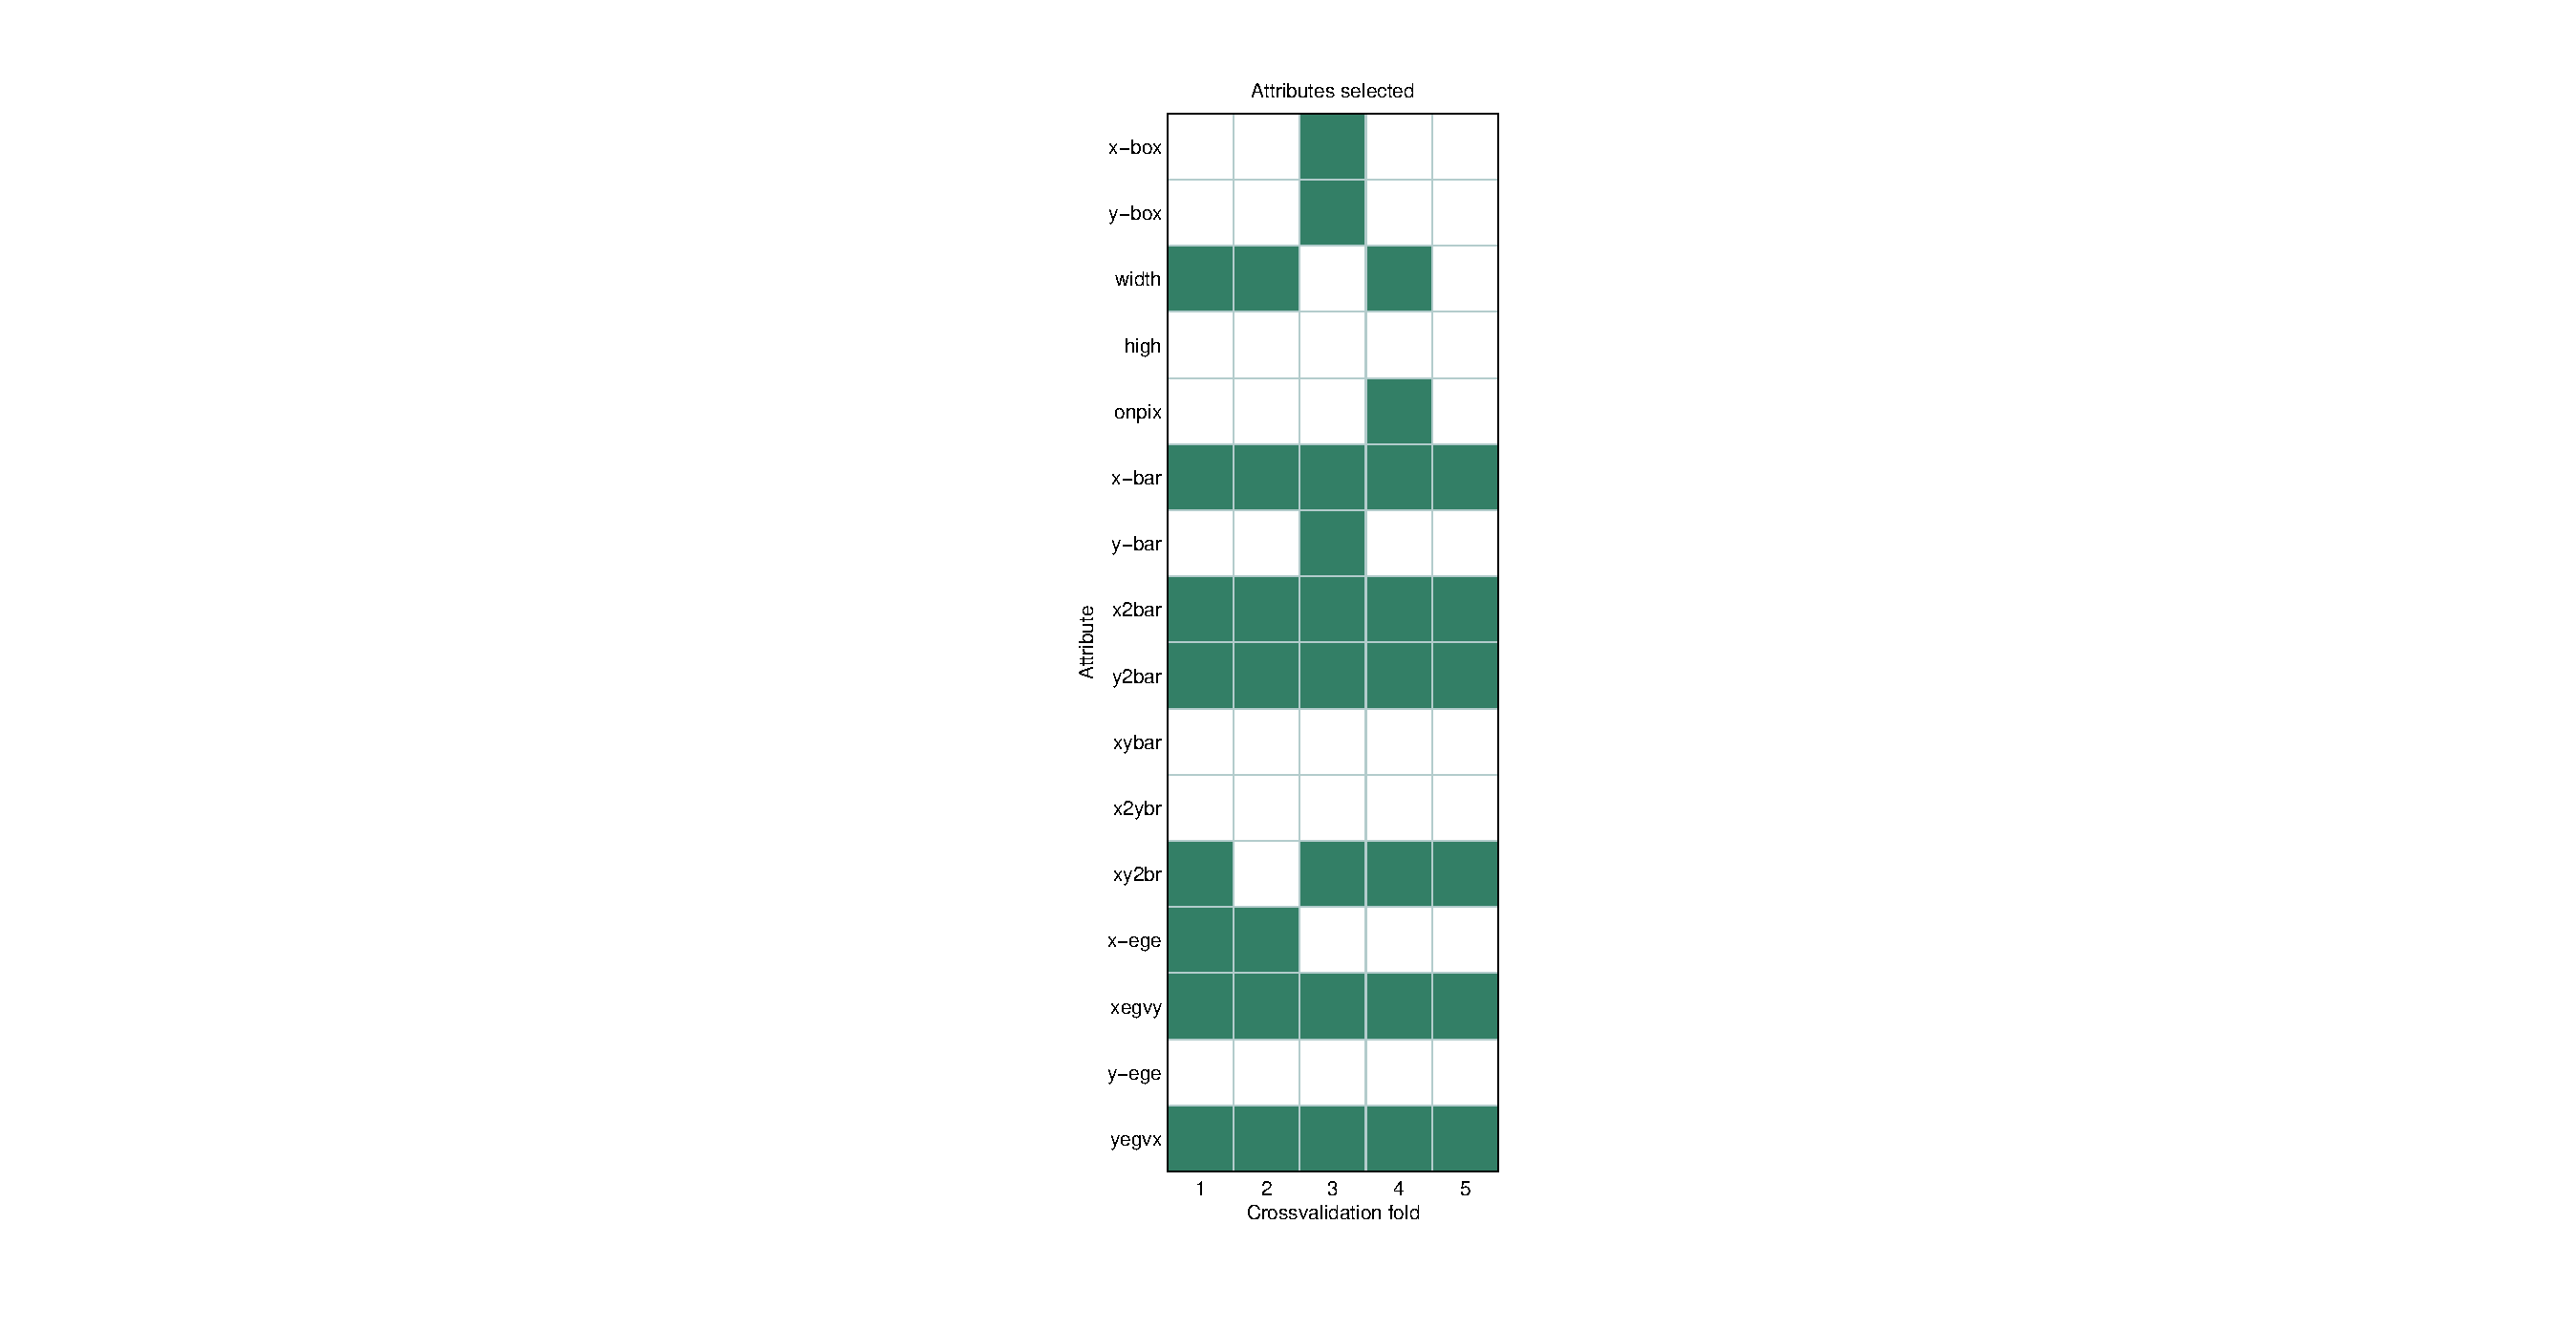
\includegraphics[width = 0.9\textwidth]{figure_p2/r1.eps}
\caption{Linear regression with forward selection, attributes selected for all folds}
\end{figure}

The fold which requires the less number of feature for the linear regression is fold number 5. Figure 1.2 shows feature selection and crossvalidation error for the fold 5. We can see that the minimum squared error is reached with only six attributes.

\begin{figure}[htbp]
\center
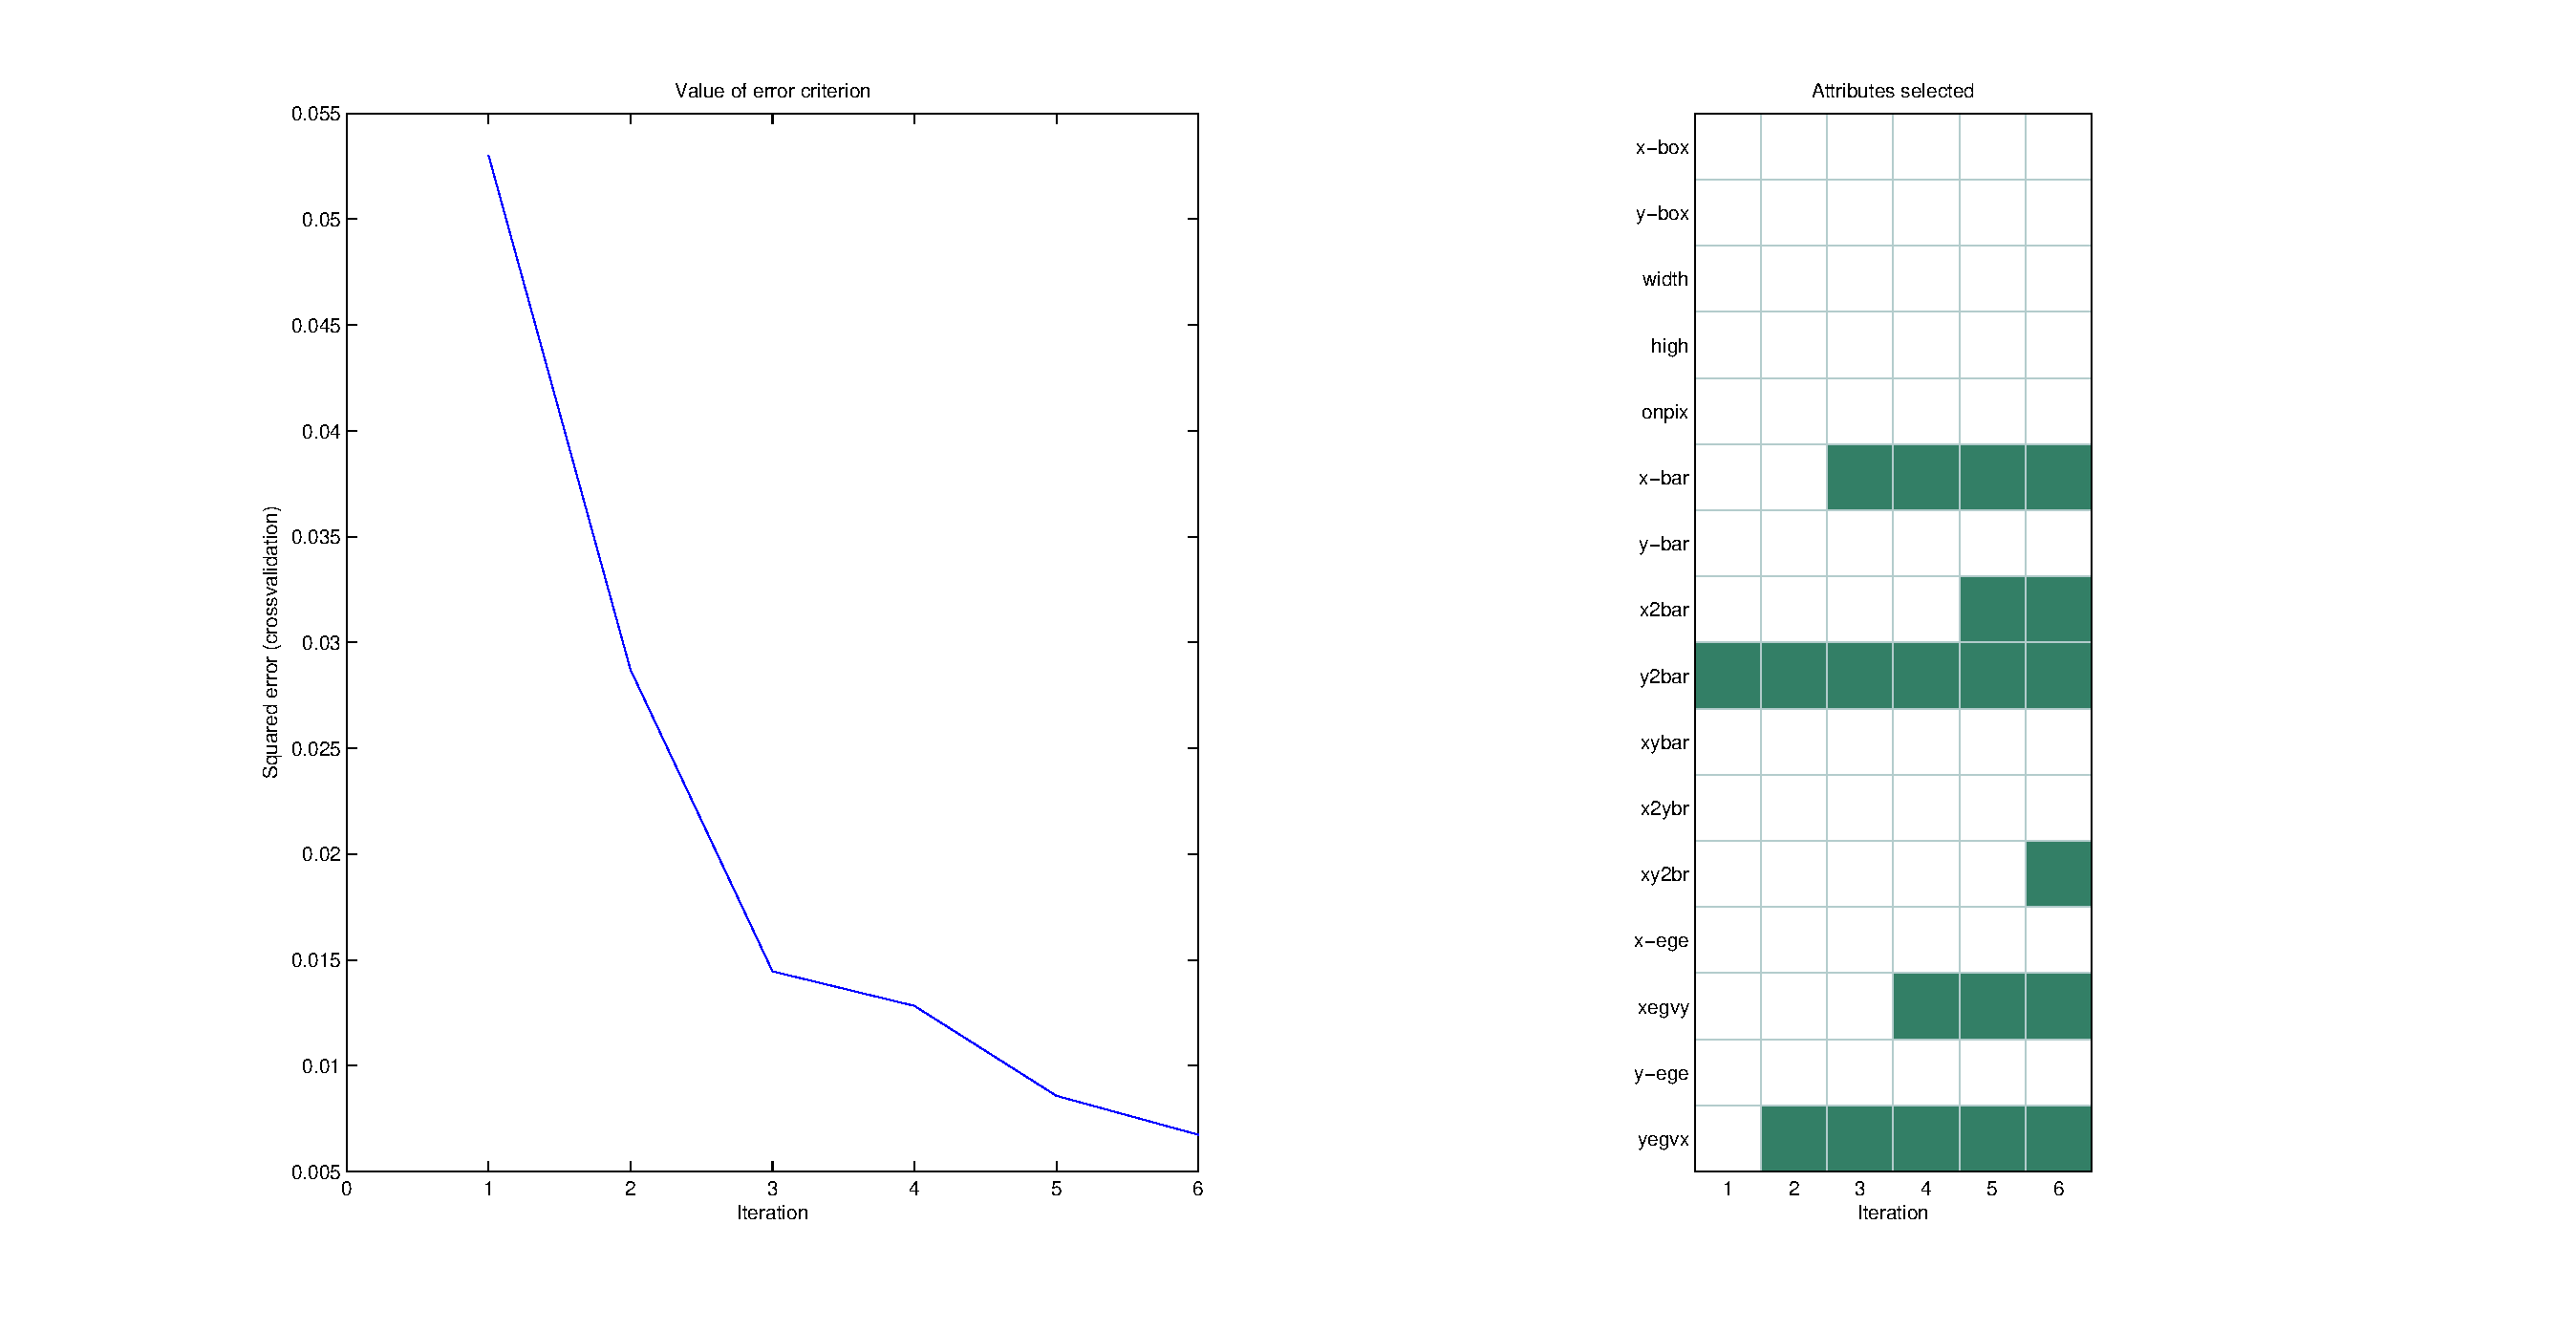
\includegraphics[width = 1.0\textwidth]{figure_p2/r2.eps}
\caption{Feature selection and crossvalidation error for fold 5}
\end{figure}

We also find that in almost all cases there is no significant performance improvement ($R^2$ test score) between selecting all the features and the features suggested by the feature selection:
\begin{verbatim}
Linear regression without feature selection:
- Training error:        0.00
- Test error:            0.01
- R^2 train:             0.99
- R^2 test:              0.95
Linear regression with sequential feature selection:
- Training error:        0.00
- Test error:            0.01
- R^2 train:             0.98
- R^2 test:              0.96
\end{verbatim}

However the feature selection allows to have a much simpler model with almost the same error performance.\\

Plotting the residual error vs. the attributes can give some insight into whether including a transformation of a variable can improve the model. If the points in a residual plot are randomly dispersed around the horizontal axis, a linear regression model is appropriate for the data; otherwise, a non-linear model is more appropriate.
Looking the residual plot in figure 1.3, it shows a random pattern which indicates a good fit for a linear model.
In fact, if we include transformation of some variable (for example the square of an attribute) we checked that there is no significant performance improvement.

\begin{figure}[htbp]
\center
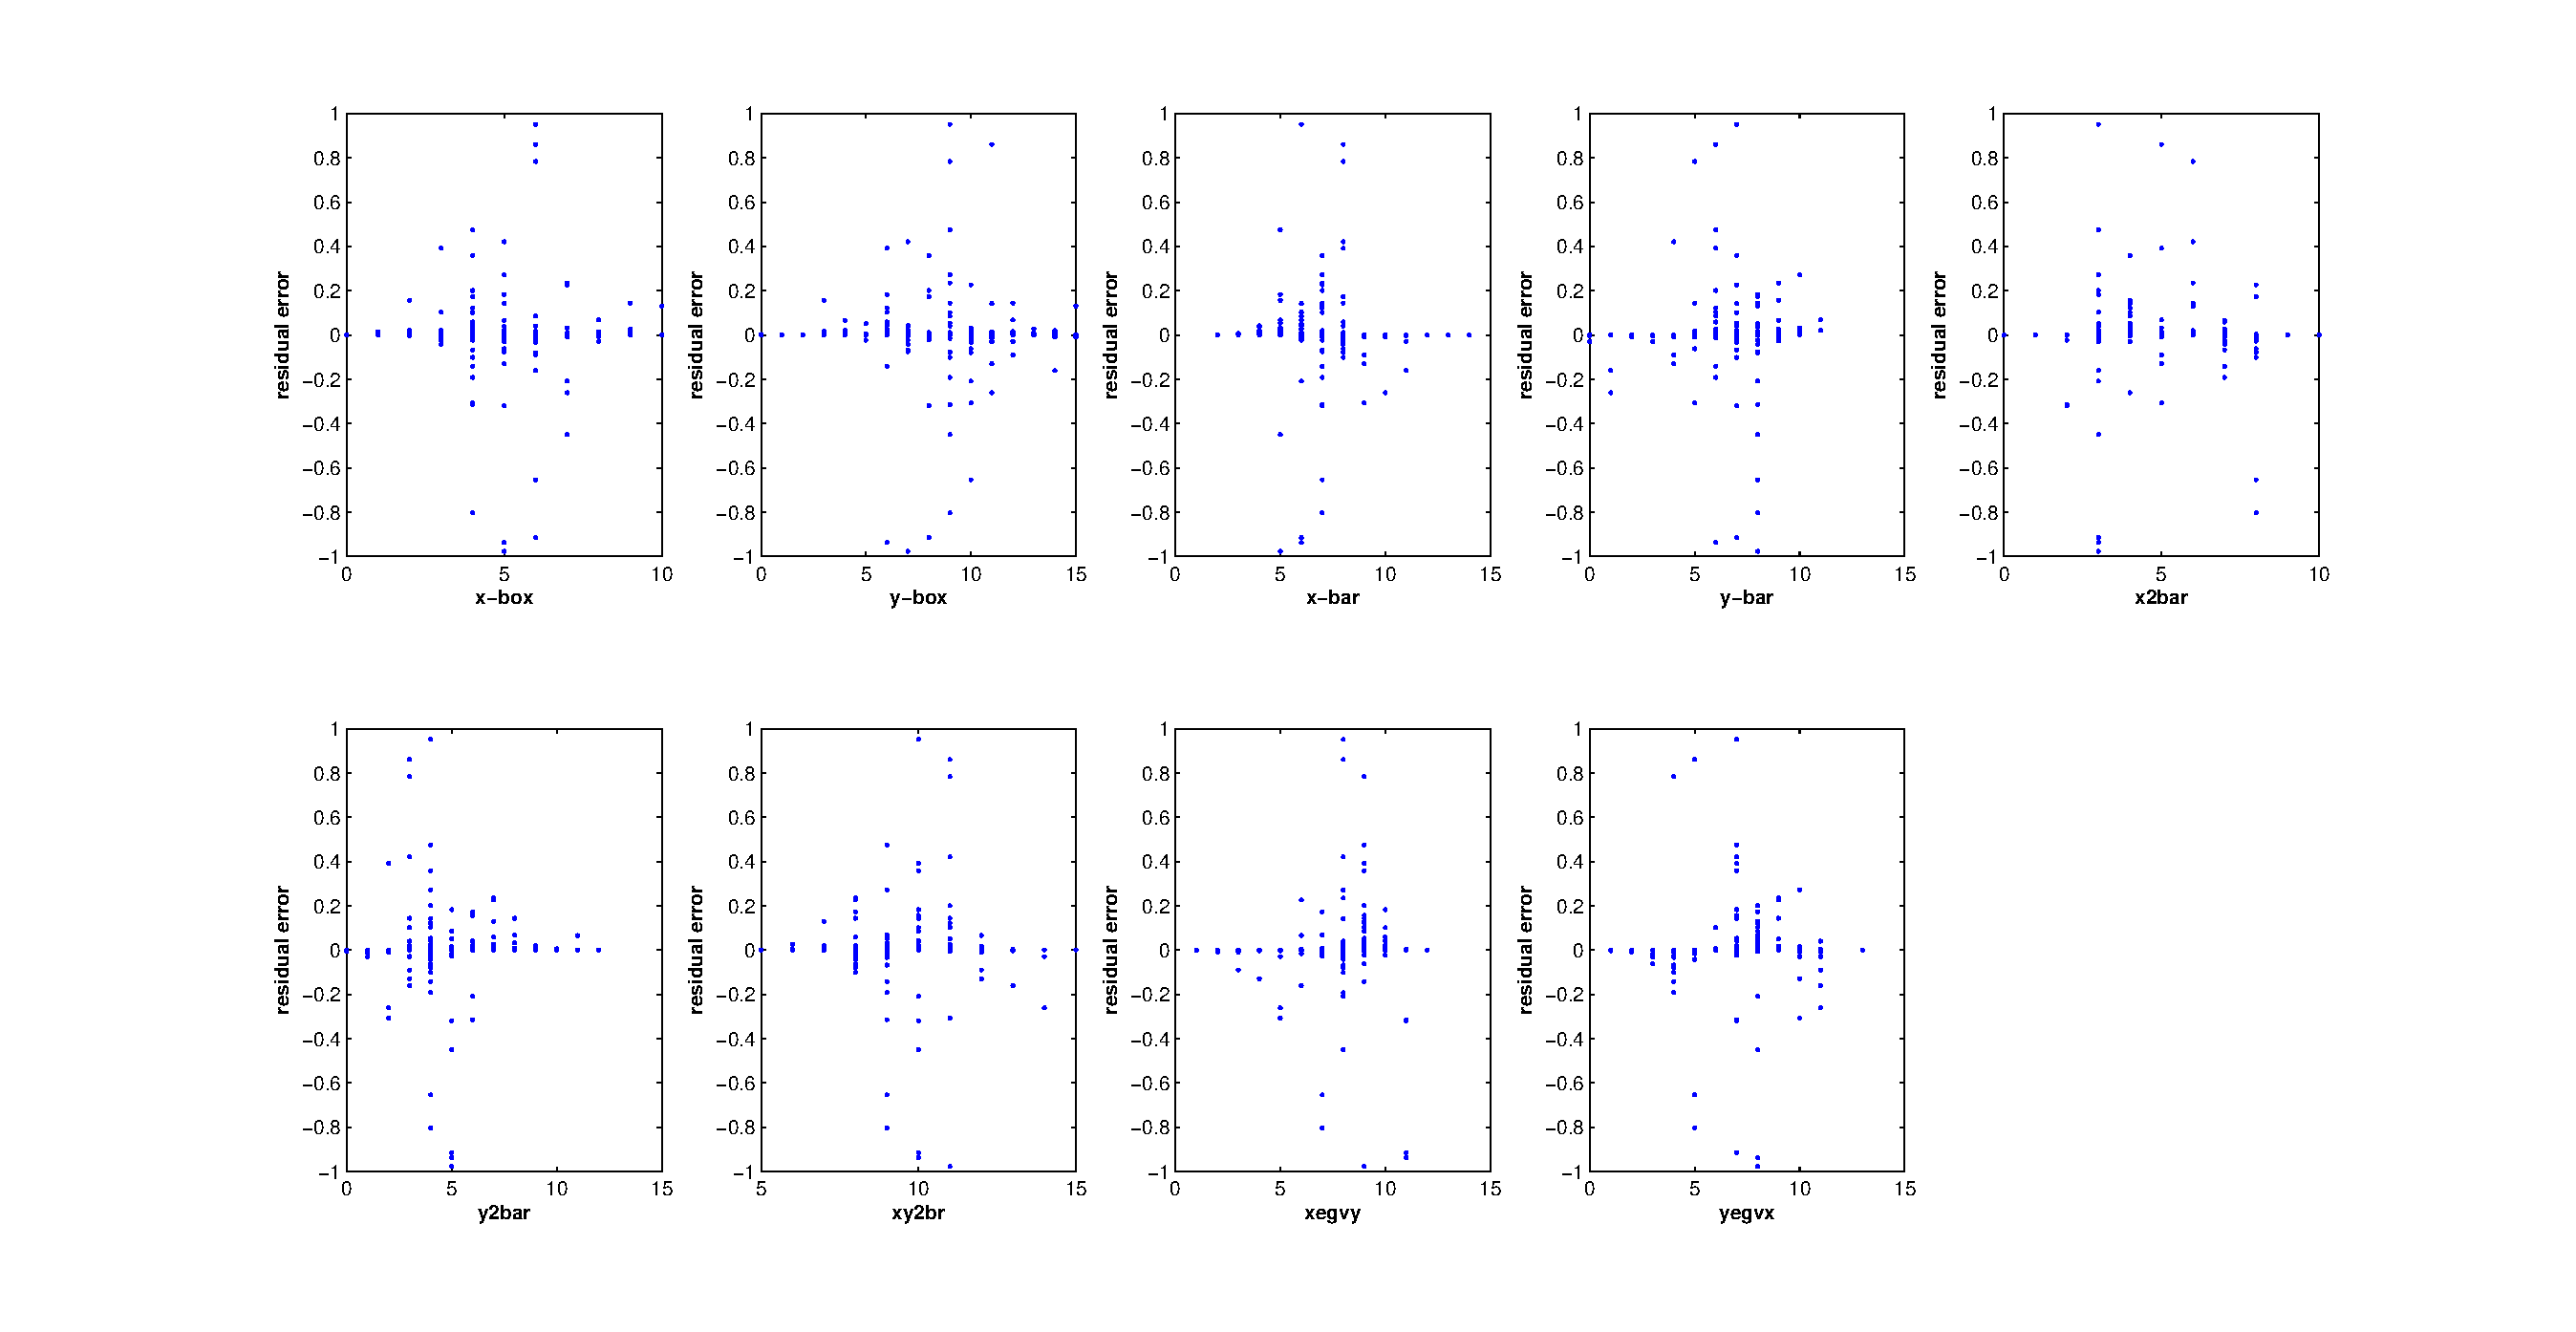
\includegraphics[width = 1.1\textwidth]{figure_p2/r3.eps}
\caption{Residual error vs. the attributes}
\end{figure}

\section*{Attributes effects}
Another approach to control for the complexity of the model is to regularize the parameters in the objective function. In linear regression we can regularize the parameter $\textbf{w}$ by the Frobenius norm. 
We run linear regression with regularization for the letter index attribute, with external 5-fold cross-validation and internal 10 fold cross-validation for estimating the optimal lambda value. Figure 1.4 shows that the optimal lambda = $10^{-2}$, and how the attribute weights change due to regularization.

\begin{figure}[htbp]
\center
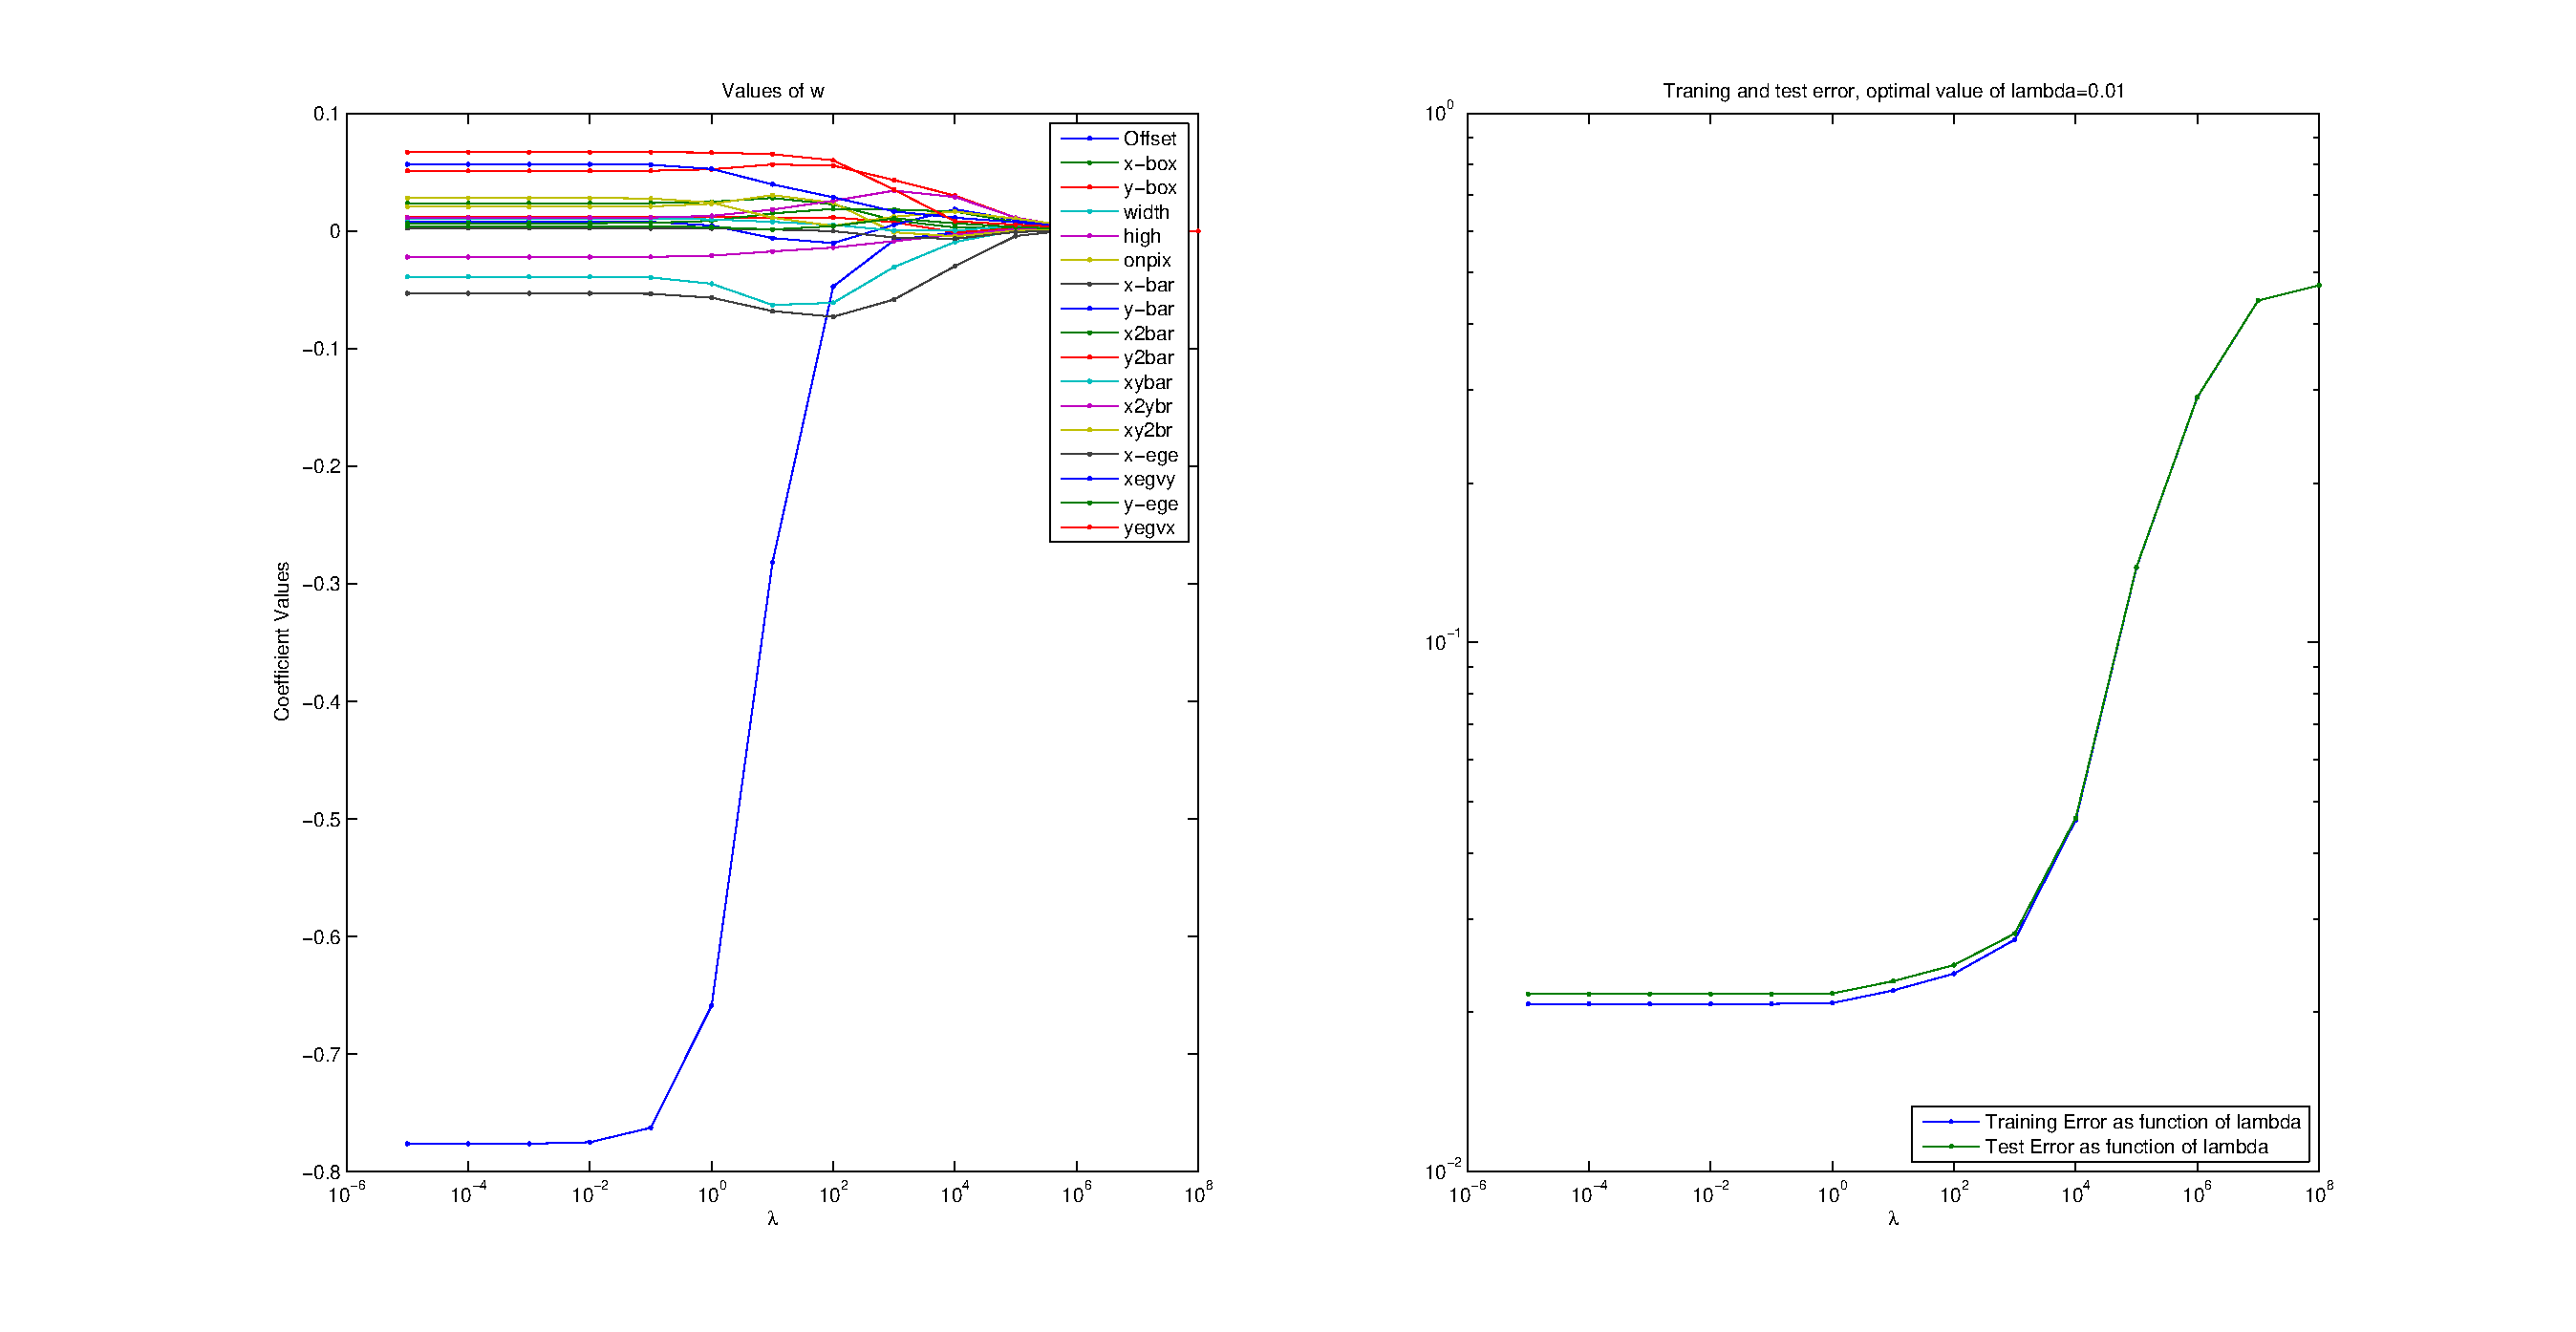
\includegraphics[width = 1.25\textwidth]{figure_p2/r5.eps}
\caption{Linear regression with regularization,  attribute weights and optimal $\lambda$}
\end{figure}

We calculate the average set of weights and we plot a bar chart to understand the contributions of the different attributes for the letter value [Figure 1.5]. We see again that in order x-bar, y2bar, xegvy, yegvx are the most significant predictors. 

\begin{figure}[htbp]
\center
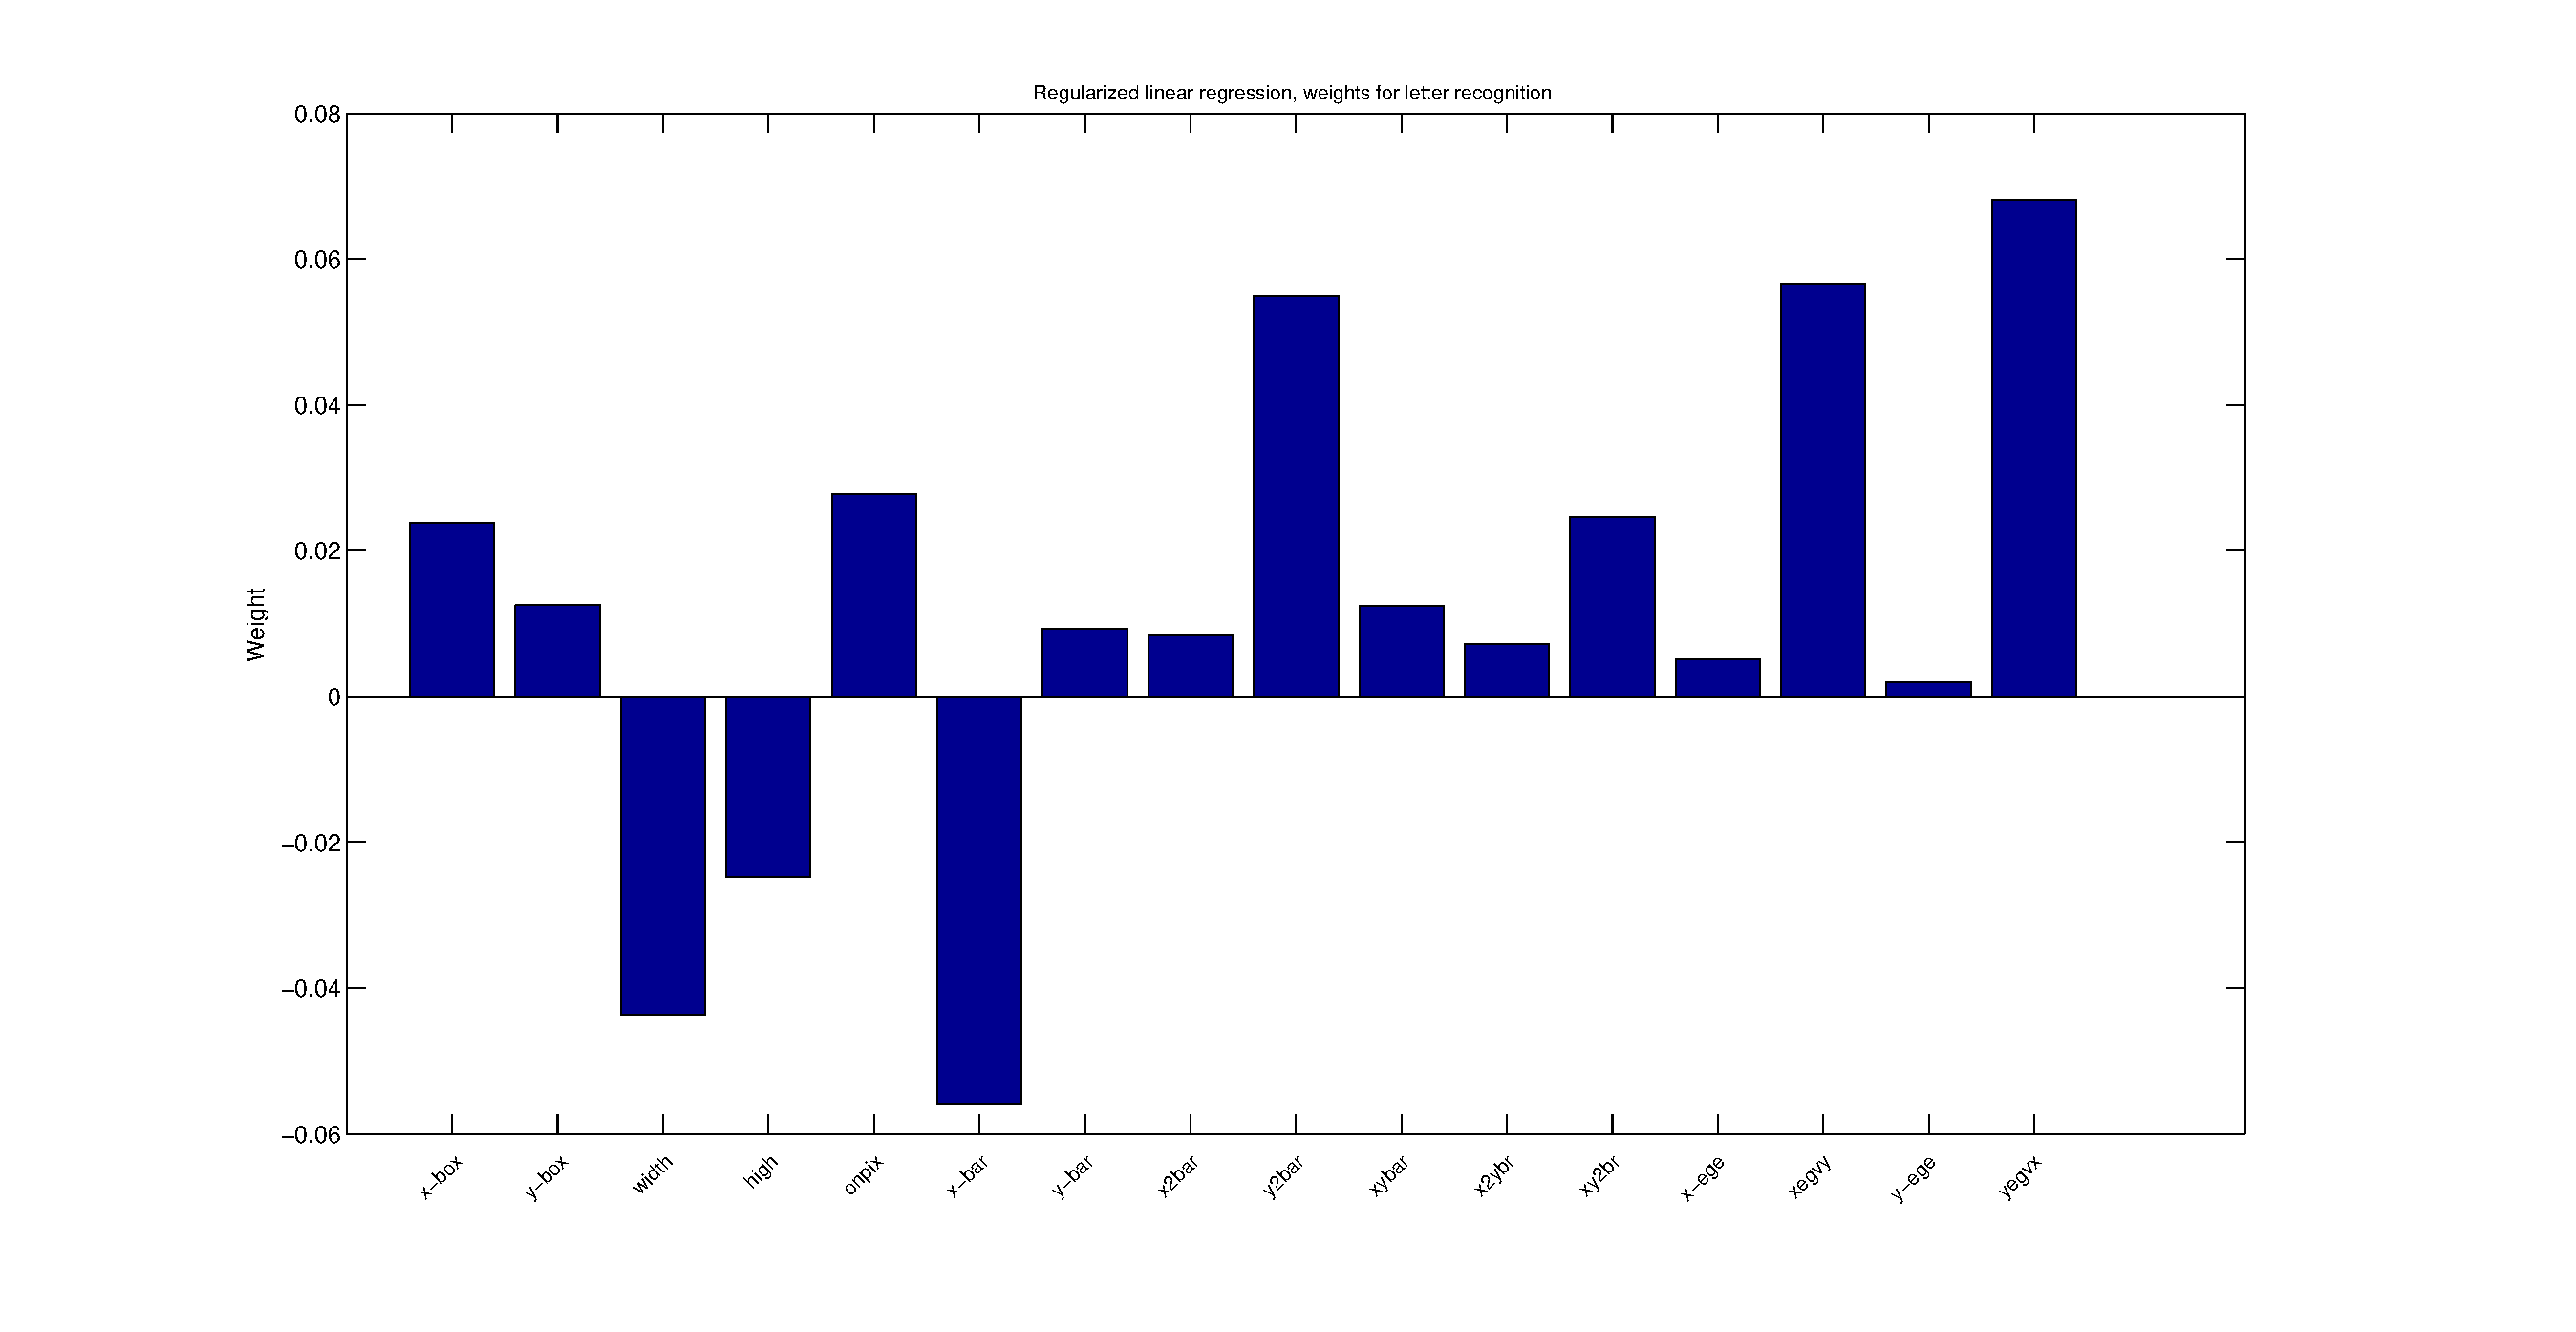
\includegraphics[width = 1.25\textwidth]{figure_p2/r6.eps}
\caption{Linear regression with regularization, attribute weights}
\end{figure}

The squared errors scores however show no significant improvement between the non regularized and the regularized models.

\section*{1.4 Artificial neural network}
We fit an artificial neural network (ANN) to the data. We perform a 5 fold cross-validation to select the number of hidden units hyper-parameter. For each fold, we try to fit an ANN 5 times, and we select the ANN which produces the lowest train error.
Just using only one hidden units and one train of neural network we obtain very interesting results, indeed, in this case, the train error and test error are approximately equal to 0\% and 1\% respectively. Increasing the number of re-train the errors remain pretty the same while increasing the number of hidden nodes (for instance equal to six), the train error and test error decrease and they are approximately equal to 0\% and 0\% (0.16\%) respectively.

Figure 1.5 describe an ANN with 16 inputs(attributes) and one hidden layer that we have chosen as model to fit our data.
\begin{figure}[htbp]
\center
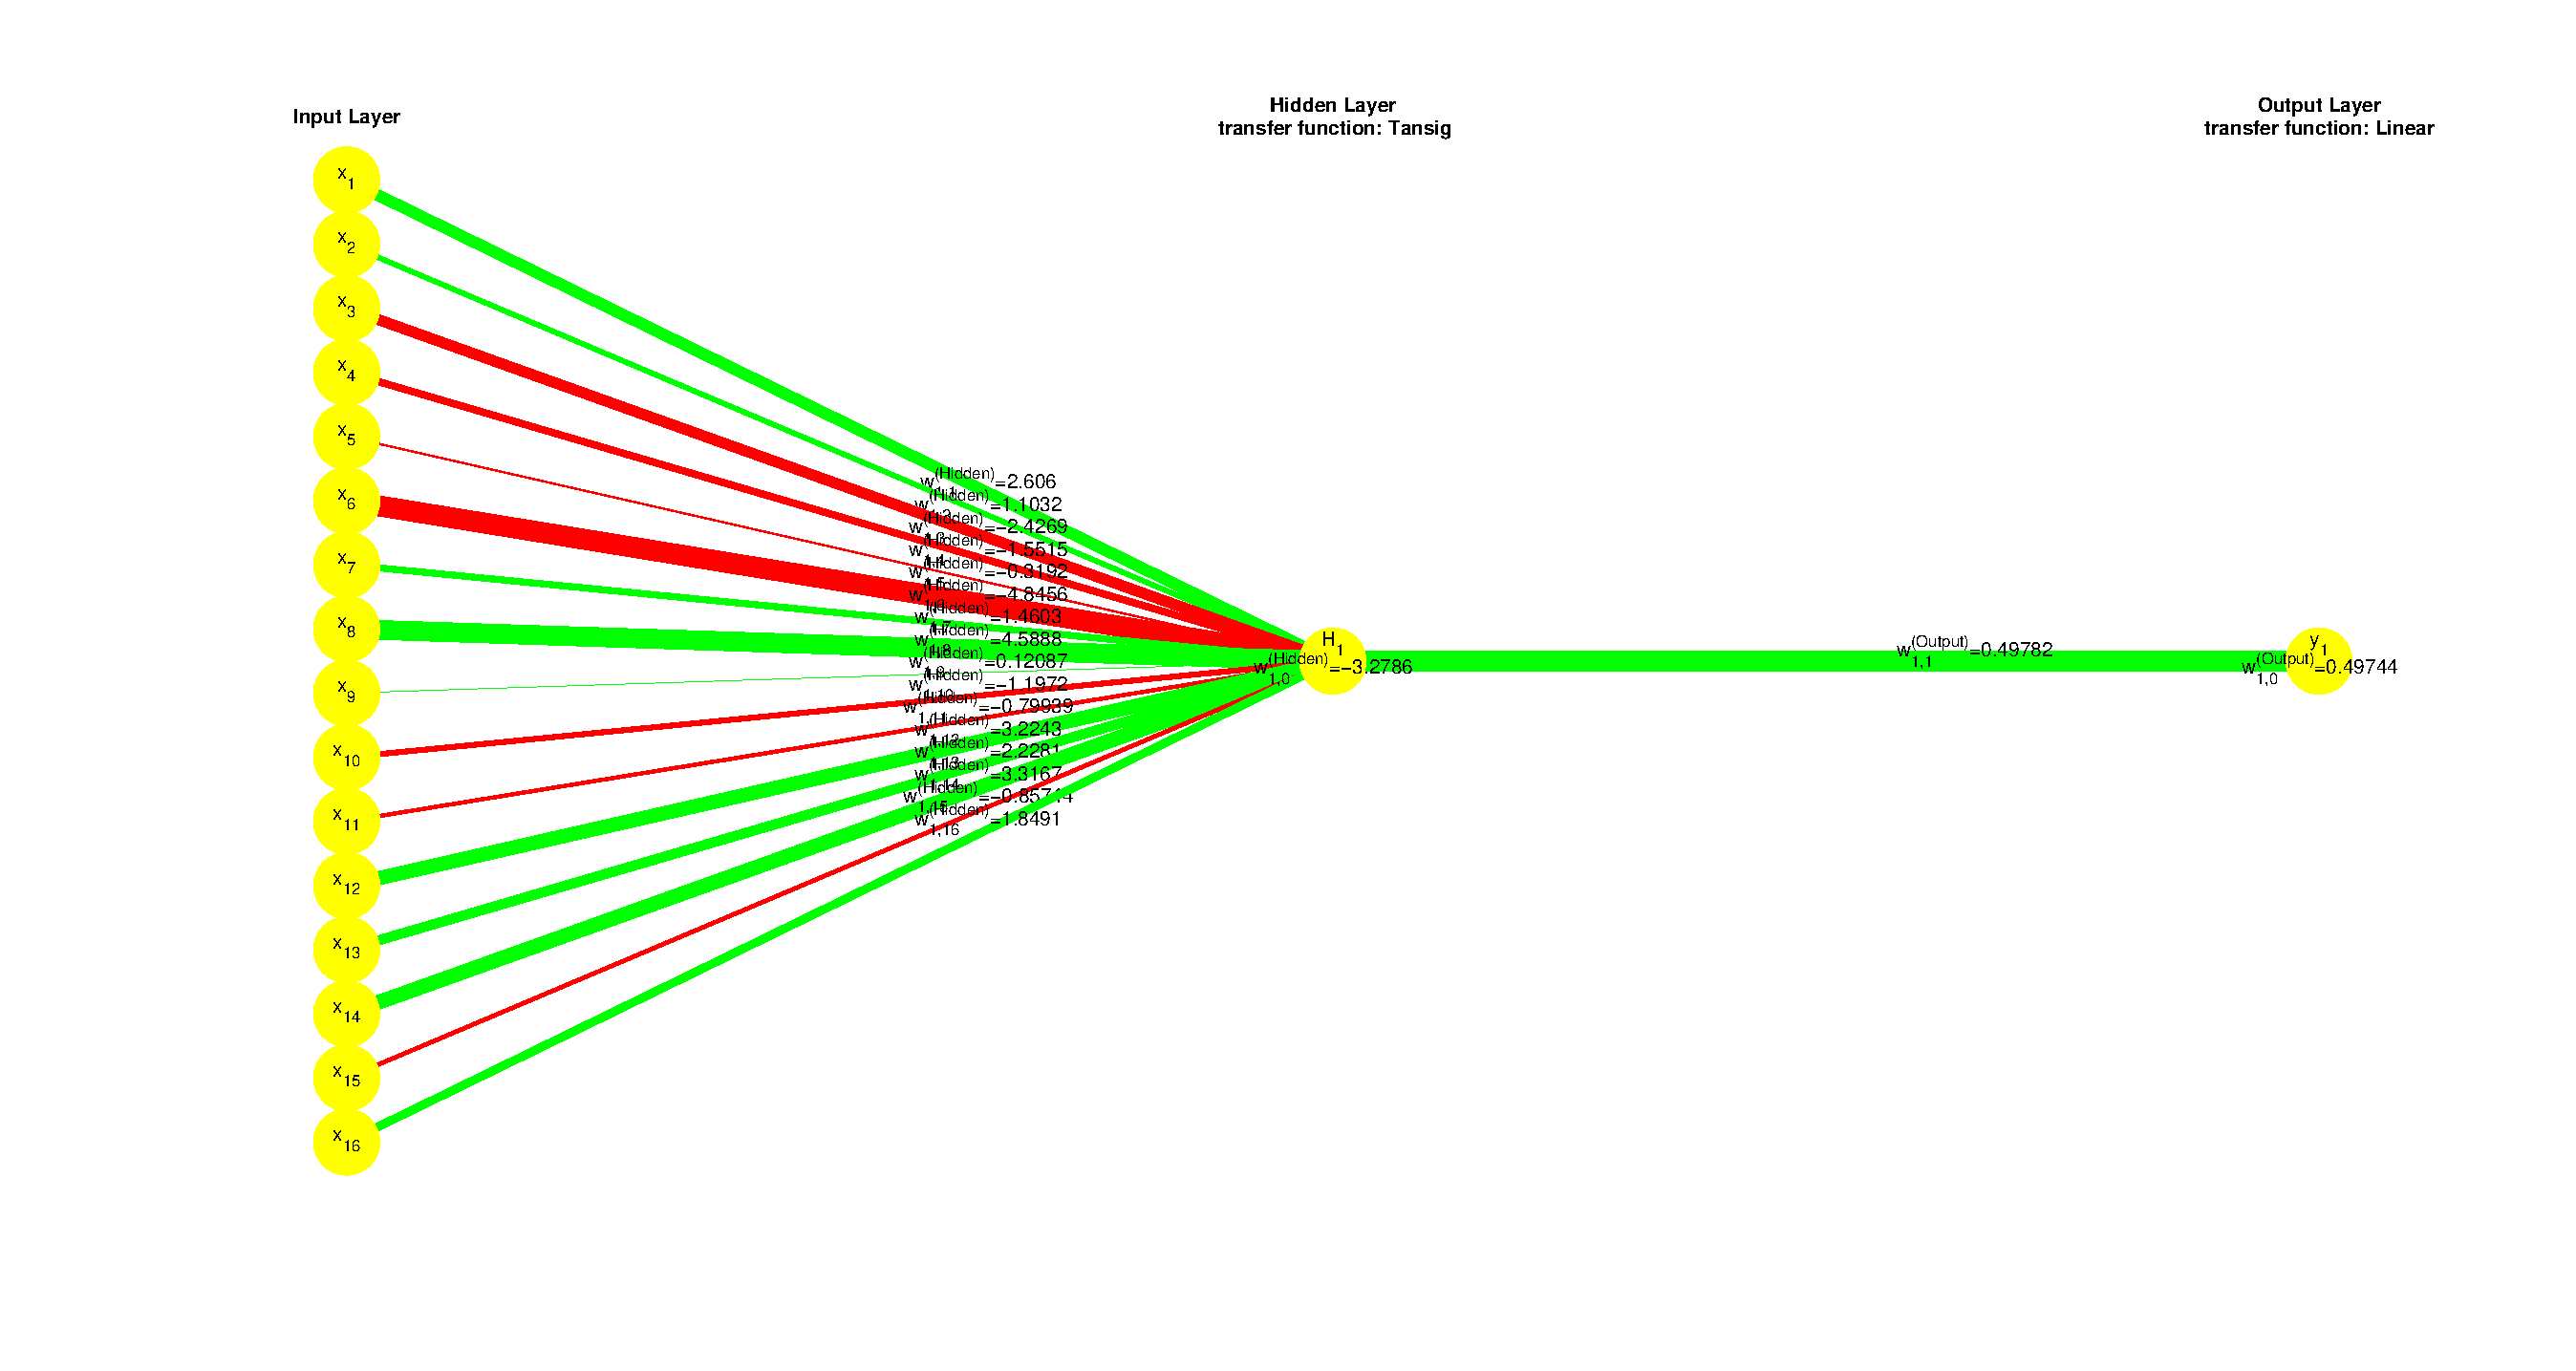
\includegraphics[width = 1.0\textwidth]{figure_p2/n1.eps}
\caption{ANN with one hidden unit}
\end{figure}


\section*{1.5 Comparison}
We perform a pairwise $t$-test between the regularized linear regression model, the ANN with one hidden node, and a baseline model predicting the average of the output variable (letter $A$ or $C$). In order to compare the models we consider the error rate average of the five folds. 
\begin{verbatim}
- Error rate linear regression      0.9%
- Error rate ANN                    1.1%
- Error rate predict average        48.3%
\end{verbatim}
If we compare Linear regression vs ANN we note that the classifiers are NOT significantly different while if we compare linear regression vs predict average and ANN vs predict average it easy understand that the classifiers are significantly different. We can see the results also in Figure 1.7.

\begin{figure}[htbp]
        \center
       	\begin{subfigure}[a]{0.35\textwidth}
                \includegraphics[width=4.8cm]{figure_p2/c1.eps}
                \caption{Linear Regression vs ANN}
        \end{subfigure}%
        \begin{subfigure}[b]{0.35\textwidth}
                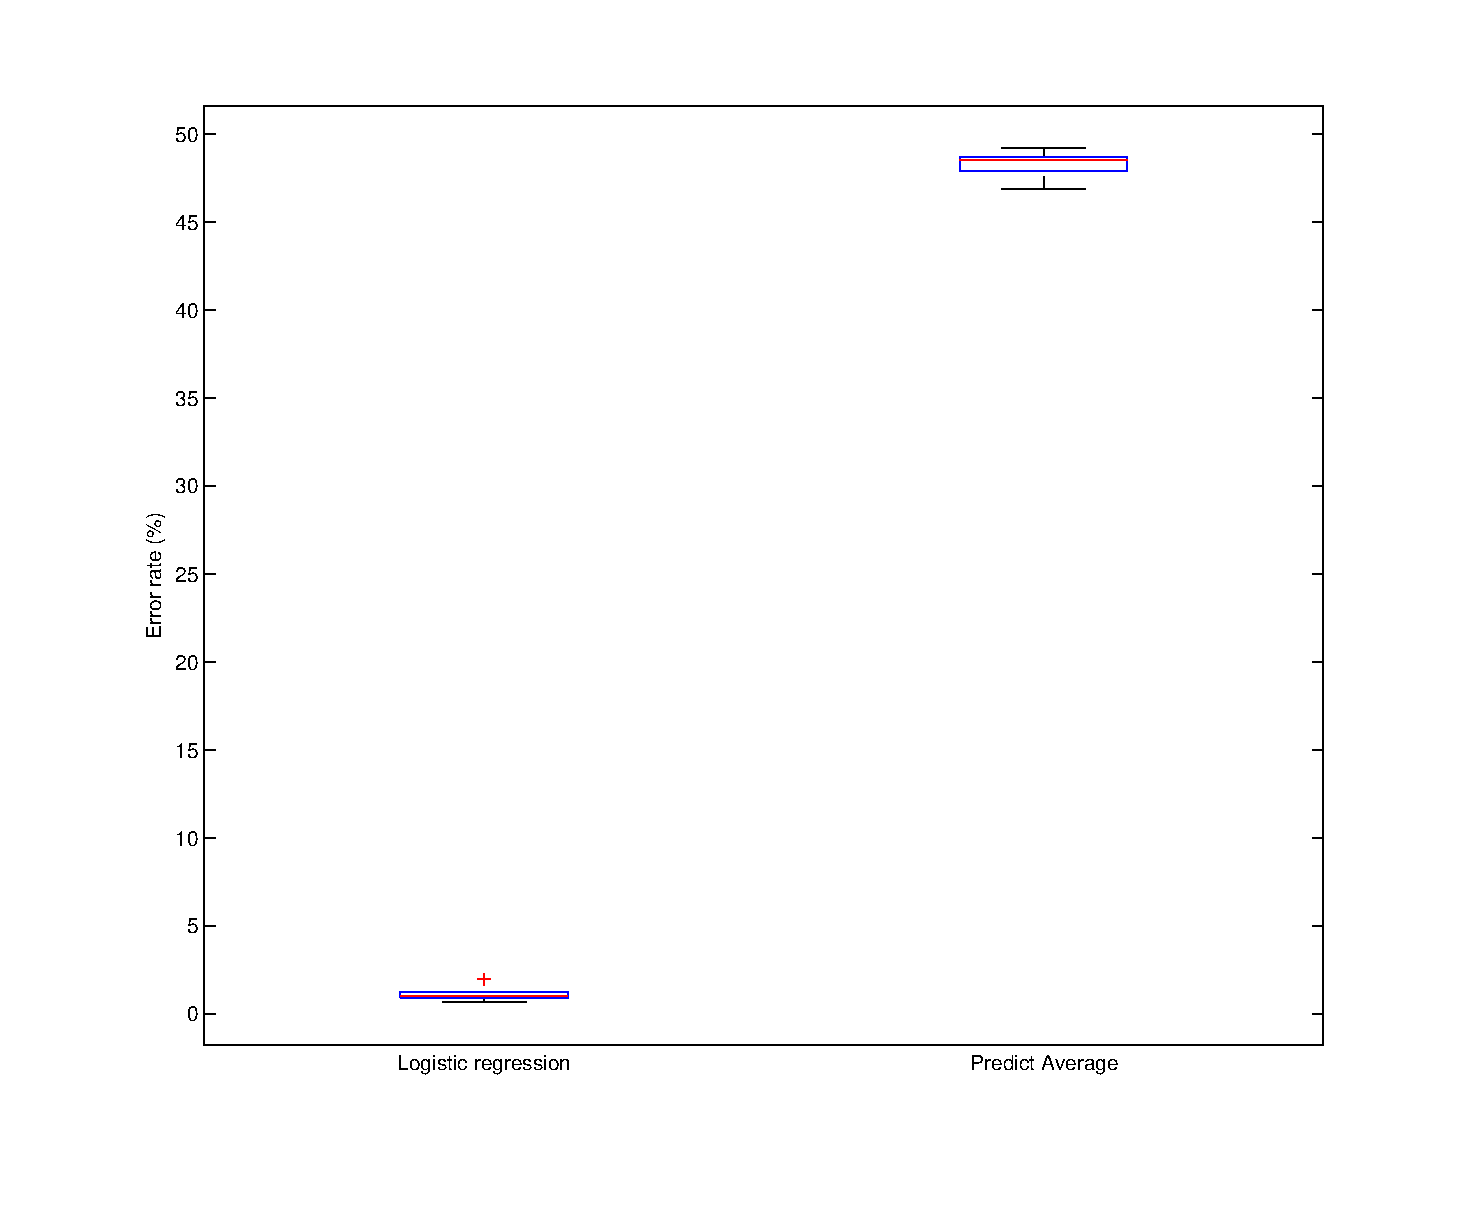
\includegraphics[width=4.8cm]{figure_p2/c2.eps}
                \caption{Linear Regression vs Predict Average}
                 \end{subfigure} \\

         \begin{subfigure}[c]{0.35\textwidth}
                \centering
                \includegraphics[width=4.8cm]{figure_p2/c3.eps}
                \caption{ANN vs Predict Average}
        \end{subfigure}
        \caption{Box-Plots: Permormace of the models one against the other}
\end{figure}

\section*{MULTI-CLASS LOGISTIC REGRESSION}
We run multi-class classification data set which fits logistic regression models to the training data using the one-against-rest strategy (each classifier trained to predict one class label vs. the remaining). Next, it computes the outputs of the C classifiers on the test data and classifies it according to the highest output.
Our goal is classify, using multi-class regression model, all the letter indexes. 

We use $\frac{2}{3}$ of the data set as training set and the remainder data for the test set and we obtain an error rate equals to 28\%.
Always considering the one-against-rest scheme, we fit 26 (number of outputs) neural networks with 2 hidden units. We use $\frac{2}{3}$ of the data set as training set and the remainder data for the test set and we obtain an error rate equals to 25\%.
Instead, considering a predict average model for all the 26 letters we obtain an error rate equals to 98\%. 
Comparing these results we can say, even in multi-class classification, that the performance of multi-class regression vs multi-class ANN are not significantly different while if we consider predict average model vs regression or ANN obviously the performance are significantly different. This happens because predict average model is very inefficient when the number of classes is high.

\chapter*{Classification}
\setcounter{chapter}{2}

\section{Problem}
The classification problem for our data we have chosen to solve is predicting a letter
from the english alphabet (26 classes) using its attributes. Each record (letter) has 16 integer
attributes in a range of 0 to 15. 
\section{Methods and parameters}
We solved this problem using KNN, ANN and Naive Bayes methods. For every method we implemented
two levels of cross-validation for estimating optimal parameters. For KNN it was a value of K, in ANN a number
of nodes in the hidden layer, and i Naive Bayes method we estimated a number of features (best) used. 
\subsection{K-Nearest Neighbors}
KNN algorithm predictions are very accurate for various values of K, but it appears that lower values are better.
The lowest error rate is for $k=1$ despite of having no duplicates in our dataset. See figure \ref{fig:KN_kvalue}
\begin{figure}[!tbh]
	\centering
	\includegraphics[width=0.9\textwidth]{figures/KN_kvalue}
	\caption{K-Nearest Neighbors - K vs error}
	\label{fig:KN_kvalue}
\end{figure}
\subsection{Naural Network}
For an artifitial neural network method we use a perceptron with one hidden layer which uses softmax function
on the output layer. We are optimizing number of nodes in a hidden layer. The lowest error rate occured with a
hidden nodes count of aproximetly 1.5 times a number of attributes, so about 26. This optimal number varies 
as the training subset changes in cross-validation, but still is close to that number. In the figure \ref{fig:NN_hiddennodes}
we can see an average of error rates for various hidden neurons count.
\begin{figure}[!tbh]
	\centering
	\includegraphics[width=0.9\textwidth]{figures/NN_hiddennodes}
	\caption{Neural Network - hidden nodes vs error}
	\label{fig:NN_hiddennodes}
\end{figure}
\subsection{Naive Bayes}
For Naive Bayes method we tried to estimate optimal features set (number of features), however no matter of what
classifier we used for feature selection using recursive feature elimination with cross-validation, the best accuracy was
obtained with selecting all features. In a plot (figure \ref{fig:NB_feature_selection}) we can see how accuracy of the method 
depends on number of features.
\begin{figure}[!tbh]
	\centering
	\includegraphics[width=0.9\textwidth]{figures/NB_feature_selection}
	\caption{Naive Bayes - features vs accuracy}
	\label{fig:NB_feature_selection}
\end{figure}
\section{Results}
For all methods, the error rate of predicting a letter basing of its attributes is below 50\%, what is quite a good result for
such a problem. The best results we got using K-Nearest Neighbors algorithm which with euclidesian mertic obtained less
than 5\% of bad answers (figure \ref{fig:performance}). Out error rate is calculated as: \\
error\_rate = (predicted\_letters != actual\_letters) / number\_of\_tests

\begin{figure}[!t]
	\centering
	\includegraphics[width=0.85\textwidth]{figures/performance}
	\caption{Performance of methods in outer cross-validation loop}
	\label{fig:performance}
\end{figure} 
\begin{figure}[!t]
	\centering
	\includegraphics[width=0.85\textwidth]{figures/predictions}
	\caption{Predicted values vs actual values (KNN)}
	\label{fig:predictions}
\end{figure}
In the figure \ref{fig:predictions} we can see a plot describing how good letters are predicted by KNN method. 
From 5000 points used only a few are away from $x=y$ line. Most of the points are on that line, which means that
letters are predicted correctly. \\

Moreover, fitting our methods for all of the data (20000 records) we obtained on average 4\% of an error rate for KNN and 35\%, 44\% 
for Neural Network and Naive Bayes accordingly. We used K-fold cross-validation using all that data which forced us to use parallelism
computing every fold in a separate thread. 
\section{Comparison}
The boxplot below (figure \ref{fig:cross_errors}) shows that there are great differences between a performance of used methods. 
\begin{figure}[!tbh]
	\centering
	\includegraphics[width=0.9\textwidth]{figures/cross_errors}
	\caption{Cross-validation errors for all methods}
	\label{fig:cross_errors}
\end{figure}
We used also a paired t-test to compare selected methods with each other and additionally with a fake predictor, which 
classifies all outputs to be the largest class in the training data: \\
\begin{tabular}{l*{4}{c}r}
Compared alg. & t-test value & p-value & significantly \\
ANN vs Naive Bayes & -10.3 & 0.0 & True \\
ANN vs KNN & 57.8 & 0.0 & True \\
Naive Bayes vs KNN & 100.5 & 0.0 & True \\
Biggest Class vs ANN & -100.4 & 0.0 & True \\
Biggest Class vs KNN & -380.7 & 0.0 & True \\
Biggest Class vs Naive Bayes & -133.3 & 0.0 & True \\
\end{tabular} \\
The results shows us that all of the methods are significantly different in case of performance.
\section{Related work}
This dataset was used for letter recognition (classification) using Holland-style Adaptive Classifiers. The article is available on the following link: \\
\url{http://download.springer.com/static/pdf/733/art%253A10.1007%252FBF00114162.pdf?auth66=1414859976_6267eff4e2e0779ac8c3bd5c7c57b61c&ext=.pdf} 
The percentage of correct identifications they achieved varies between 50\% to 80\% depending on the settings, where the highest score is
obtained with the most computationally demanding settings. Refering to that article we can assume that our results are successful. 






\chapter*{Conclusions}
Summing up our work, we observed that K-Nearest Neighbors algorithm is the best method for letter
classification on our dataset. Neural networks also gained good results, however they could be made
more precise applying deep neural networks with doing computations on GPU. Some of our methods
were a way better than these presented by previous researchers. 

%\chapter*{Preface} 
Preface text\dots

%\chapter{Testing}
\section{Images}
Always have images/figures in \emph{both} EPS and PDF/PNG/JPG format! (unless you know you only will be using pdfLaTeX)


\begin{figure}[!tbh]
	\centering
	\includegraphics[width=0.5\textwidth]{testimage}
	\caption{Test of image insertion.}
	\label{fig:testimage}
\end{figure}

\section{Tables}
\begin{table}[!h]
\centering%
\caption{Simple table.}\label{tab:table}
\begin{tabular}{| r l |}
   \hline
   aaaaaaaaaaaaaaa & bbbbbbbbbbbbb\\
   c & d\\
   \hline
\end{tabular}
\end{table}

\section{References} References are made with `\ref{tab:table}'. Refer to a page with 
`\pageref{tab:tabel}'.

\section{Bibliography} \cite{Deitel:2002} is a reference to a book.
%\bibliographystyle{plain} % pr�v ogs�: is-unsrt, alpha, plain
\bibliography{biblio/template-bib}
%\nocite{*} % \nocite bruges til b�ger som skal med i litteraturlisten
            % men som ikke er refereret til. Alts� baggrundsstof mv.


%\appendix % Alphabetic chapter numbering
%\renewcommand{\appendixtocname}{Appendix} % Change appendix name for the table od contents
%\addappheadtotoc % 'Appendix' to the table of contents
%\chapter{Appendix}
Insert your appendix here.
%\backmatter % for glossary, index, back page
\end{document}
